\documentclass[a4paper,french]{paper}
\usepackage{../../../../../_assets/latex/5N_OPTO_ELEC}

%Informations about this document 
%------------------------------------------
\def\module{Opto-Electronique - S5}
\def\moduleAbrege{5N-027-SCI / OptoElec}
\def\annee{2024-2025}

\def\titre{Séance 2 / Capteurs et mise en forme}
\author{Julien VILLEMEJANE}

\subtitle{Séance 2}
\institution{LEnsE / Institut d'Optique Graduate School}

\title{\titre}
\begin{document} 
%Beginning First Page. 
%------------------------------------------
\enteteThematiqueObligatoire{}

\textit{Pour ce TD, on pourra s'appuyer sur la fiche résumée} : \href{https://lense.institutoptique.fr/ressources/Annee1/Electronique/fiches/2021_FR_ALI.pdf}{Ampli Linéaire Intégré}.

%Beginning Content. 
%------------------------------------------


%%%%%%%%%%%%%%%%%%%
\encadreTDExo{2.1 - Élever une tension}{
Proposez un circuit permettant d'élever une tension d'un facteur $k$.

$k > 1$
}

%%%%%%%%%%%%%%%%%%%
%%%%%%%%%%%%%%%%%%%
\encadreTDExo{2.2 - Amplifier un signal}{
Proposez un circuit permettant d'amplifier un signal de $27dB$, tout en garantissant une bande-passante de $400 kHz$.

On utilisera des amplificateurs linéaires intégrés de type TL081 (documentation partielle donnée en annexe du TD1).
}

%%%%%%%%%%%%%%%%%%%
%%%%%%%%%%%%%%%%%%%
\encadreTDExo{2.3 - Additionner des signaux}{
On se propose d'étudier le circuit suivant :

\begin{center}
\begin{circuitikz} 
	\node [op amp, fill=blue!10!white](A1) at (0,0){\texttt{AOP1}};
	\draw (A1.-) to[short] ++(-.5,0) coordinate(A) to[short, -*] ++(0,1.5) coordinate(B) to[R=$Z_S$] (B -| A1.out) to[short, -*] (A1.out);
		
	\draw (A1.-) to[short,-*] ++(-.5,0) coordinate(AA) to[R=$Z_1$] ++(-2.5,0) coordinate(BB) to[short,-o] ++(-.5,0) coordinate(CC);
	
	\draw (B) to[R=$Z_i$] ++(-2.5, 0) to[short, -o] ++(-1.5, 0);
	
	\draw (B) -- ++(0, 1.5) to[R=$Z_N$] ++(-2.5, 0) to[short, -o] ++(-2.5, 0);	
	
	\draw (A1.+) to[short] ++(0,-0.5) node[ground]{};
	\draw (A1.out) to[short,-o] ++(1,0) coordinate(D);
	\draw (-4.6,-1) edge[->,color={green!40!black}] (-4.6,0.3);
	\node[text={green!40!black}] (Ve) at (-5.1,-0.35){$V_{e1}$};		\draw (-4.6,-1.3)  to[open,-o] ++(0,0) node[ground](GND){};


	\draw (-5.6,-1) edge[->,color={green!40!black}] (-5.6,1.7);
	\node[text={green!40!black}] (Ve) at (-6.1,0.65){$V_{ei}$};	
	\draw (-5.6,-1.3)  to[open,-o] ++(0,0) node[ground](GND){};
	
	\draw (-6.6,-1) edge[->,color={green!40!black}] (-6.6,3.1);
	\node[text={green!40!black}] (Ve) at (-7.1,1.35){$V_{eN}$};	
	\draw (-6.6,-1.3)  to[open,-o] ++(0,0) node[ground](GND){};
	 
	
	\draw (2.2,-1) edge[->, color={red}] (2.2,-0.3);
	\node[text={red}] (Vs) at (1.7,-0.6){$V_s$}; 
	\draw (2.2,-1.3)  to[open,-o] ++(0,0) node[ground](GND){};
	
\end{circuitikz}
\end{center}

}

%%%%%%%%%%%%%%%%%%%
%%%%%%%%%%%%%%%%%%%
\encadreTDExo{2.4 - Mettre en forme un capteur de température}{
On se propose d'étudier le circuit suivant :

\begin{center}
	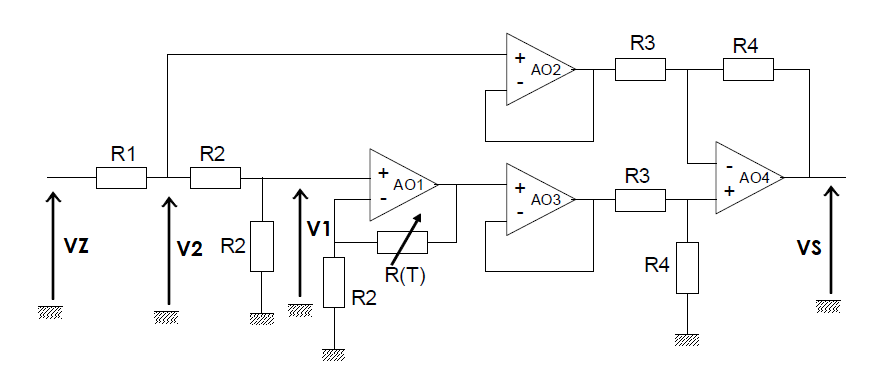
\includegraphics[width=16cm]{images/capteur_conditionnement.png}
\end{center}

La thermistance utilisée est de type PT100. La relation entre sa résistance (en Ohms) et la température (en \degre{}C) est la suivante :
$$R(T) = 100~(1 + 3.908×10^{-3} T - 5.802×10^{-7} T^2)$$
}

%%%%%%%%%%%%%%%%%%%
%%%%%%%%%%%%%%%%%%%
\encadreTDExo{2.B1 - Pilotage TOR en fonction de la luminosité}{

\textit{TOR signifie Tout Ou Rien}

On souhaite réaliser un détecteur qui allume une LED lorsque la luminosité ambiante diminue. On propose pour cela le montage suivant qui utilise une cellule photoconductrice CdS. On donne : $V_{cc} = 12\operatorname{V}$ et $R_2 = 100\operatorname{k\Omega}$.

\begin{center}
	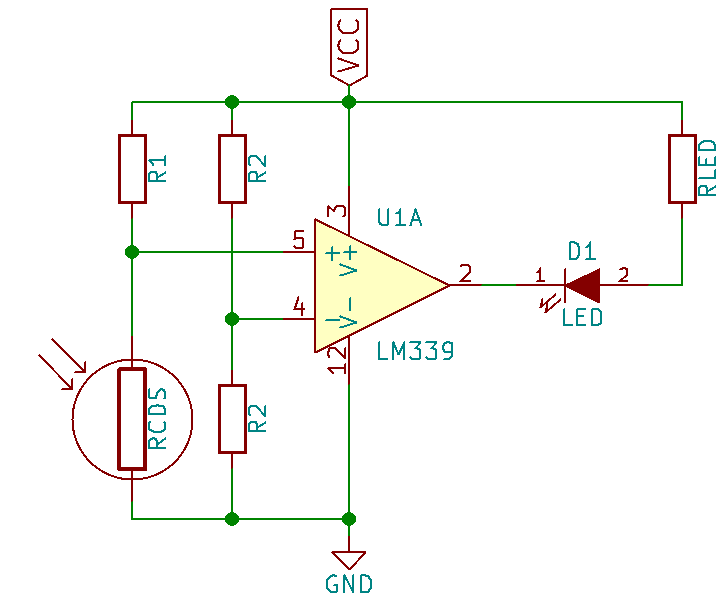
\includegraphics[width=9cm]{images/comparateur_luminosite.png}
\end{center}

On donne ci-dessous les caractéristiques de la cellule CdS.

\begin{center}
	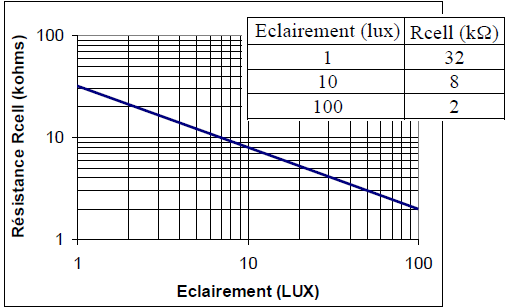
\includegraphics[width=10cm]{images/capteur_CDS.png}
	
	Caractéristique Résistance en fonction de l'Eclairement de la cellule CDS
\end{center}

On rappelle que l'amplificateur linéaire intégré, le \textbf{LM339}, est un comparateur à collecteur ouvert (voir la fiche résumée \textsc{Amplificateur Linéaire Intégré}).

\begin{enumerate}
	\item Quelle est la fonction réalisée par l'amplificateur opérationnel (AO) dans ce montage ?
	\item Dans quelle condition sur $V+$ et $V-$ la LED sera-t-elle allumée ?
	\item Calculer la tension à la sortie de la cellule CDS.
	\item Vérifier le bon fonctionnement du système.

\medskip
	
	On mesure la valeur de la photocellule ($R_{cell0} = 5\operatorname{k\Omega}$) dans des conditions d'éclairement ambiant. 
	
	\item Calculer la valeur de $R_1$ pour que la LED s'allume lorsque l'éclairement diminue d'un facteur 10.
\end{enumerate}
}

\end {document}